\documentclass[12pt]{article}

\usepackage[margin=1in]{geometry}
\usepackage{parskip}
\usepackage{amsmath}
\usepackage[backend=biber, style=alphabetic, sorting=ynt]{biblatex}
\usepackage{graphicx}
\usepackage{wrapfig}
\usepackage{float}
\usepackage{caption}
\usepackage{hyperref}

\graphicspath{{./images/}}

\begin{document}

\title{Applying State Space Control and LQR to the Pole Balancing Problem}
\author{Brendon Matusch}
\date{November 2018}
\maketitle

\section{Introduction}

\subsection{The Pole Balancing Problem}

One of the most famous problems in control theory is the \textit{pole balancing problem}, also known as \textit{cart pole}. The basic idea of the problem is as follows:
\begin{itemize}
    \item A movable cart sits on a straight, finite-length track.
    \item A pole (light, relative to the cart) is anchored to the cart with a hinge.
    \item A motor is attached to the cart; it can accelerate the cart to the left or right.
    \item The goal is to prevent the pole from falling over, while also keeping the cart near the center of the track.
\end{itemize}

\begin{figure}[h]
    \centering
    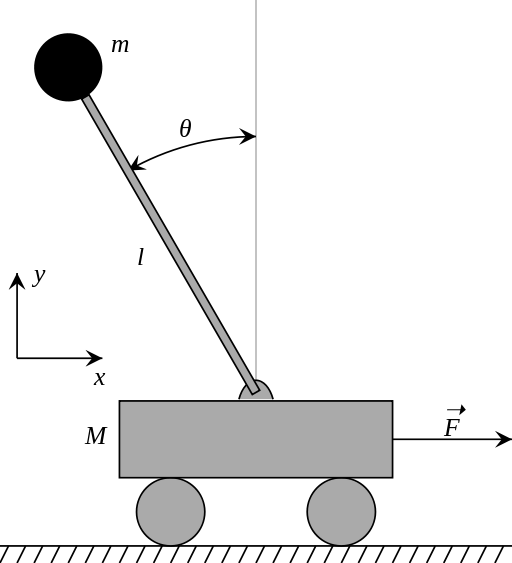
\includegraphics[width=180pt]{cartpole}
    \caption{\label{cartpole} A diagram of the pole balancing problem.}
\end{figure}

This problem is quite clearly not trivial. If the pole starts to fall to the right, one must accelerate the cart to the right to prevent it from falling over. However, that also results in the cart moving away from the center. Thus, to successfully optimize both the angle and the position, one must gradually adjust the angle by applying small forces while the cart moves.

\subsection{Control Algorithms}

The most common classical control solution to this kind of problem is the PID (proportional, integral, and derivative) closed control loop. While it is well-known that this can work, it is relatively difficult to optimize. PID loops are only able to optimize one variable at a time (for instance, the angle of the pole, or the position of the cart). Optimizing multiple variables (as is required here) necessitates nesting of PID loops, which frequently have to be optimized either manually or via machine learning.

An alternative control method, which can optimize multiple variables with one or more inputs, is state space control. Rather than dealing with only a single variable, state space controllers can optimize an entire vector of states in a single linear function, making for a simpler and more elegant solution.

For this project, I have created a mathematical simulation of the pole balancing problem and developed a state space controller to effectively optimize it.

\subsection{Applications}

A state space solution to the pole balancing problem has many applications outside of this environment. For instance, control of many kinds of robots (such as two-wheeled vehicles and walking humanoid robots) is related to the pole balancing problem. I have learned a great deal along the way about how state space control algorithms can generalize onto real-world control problems.

\end{document}